%
% File interchangeability.tex
%
\documentclass[11pt,a4paper]{article}
\usepackage[hyperref]{naaclhlt2019}
\usepackage{times}
\usepackage{latexsym}

\usepackage{url}

%\aclfinalcopy % Uncomment this line for the final submission
\def\aclpaperid{199} %  Enter the acl Paper ID here

%\setlength\titlebox{5cm}
% You can expand the titlebox if you need extra space
% to show all the authors. Please do not make the titlebox
% smaller than 5cm (the original size); we will check this
% in the camera-ready version and ask you to change it back.

\usepackage[utf8]{inputenc} % allow utf-8 input
\usepackage[T1]{fontenc}    % use 8-bit T1 fonts
\usepackage{hyperref}       % hyperlinks
\usepackage{url}            % simple URL typesetting
\usepackage{booktabs}       % professional-quality tables
\usepackage{amsfonts}       % blackboard math symbols
\usepackage{nicefrac}       % compact symbols for 1/2, etc.
\usepackage{microtype}      % microtypography
\usepackage{pgfplots,pgfplotstable}

\title{Syntactic Interchangeability in Word Embedding Models}

\author{
Daniel Hershcovich \qquad Assaf Toledo \qquad Alon Halfon \qquad Noam Slonim \\
IBM Research\\
\texttt{\{danielh,assaf.toledo,alonhal,noams\}@il.ibm.com}
}

\begin{document}
    \maketitle

    \begin{abstract}
    Nearest neighbors in word embedding models are commonly observed to be
    semantically similar, but the relations between them can vary greatly.
    We investigate the extent to which word embedding models
    preserve syntactic interchangeability, as reflected by distances between
    word vectors, and the effect of hyper-parameters---context window size in particular.
    We use part of speech (POS) as a proxy for syntactic interchangeability,
    as generally speaking, words with the same POS are syntactically valid in the same contexts.
    We also investigate the relationship between interchangeability
    and similarity as judged by commonly-used word similarity benchmarks,
    and correlate the result with the performance of word embedding models
    on these benchmarks.
    Our results will inform future research and applications in the selection
    of word embedding model, suggesting a principle for an appropriate selection
    of the context window size parameter depending on the use-case.
    \end{abstract}

    \section{Introduction}\label{sec:introduction}

    Word embedding models \cite{mikolov2013efficient,pennington2014glove,levy2015improving}
    attempt to capture the semantic space of words
    in a metric space of real-valued vectors.
    While it is common knowledge that the hyper-parameters used to train these
    models affects the semantic properties of the distances arising from them
    \cite{goldberg2016primer}, and indeed, it has been shown that
    they capture many different semantic relations \cite{yang2006verb,agirre2009study},
    little has been done to quantify the
    effect of model hyper-parameters on output tendencies.
    In this work, we begin to answer this question.
    As a test case, we experiment with fastText \cite{bojanowski2016enriching}.
    We take the context window size as the hyper-parameter,
    and syntactic interchangeability of words as the relation under investigation,
    expressed by the part of speech (POS).
    
    \paragraph{Context window size.}
    Word embedding algorithms learn vector representations for words,
    using co-occurrences from a text corpus,
    based on the distributional hypothesis \cite{harris1954distributional}.
    Co-occurrences are usually extracted by finding, for each word token, all
    words within a constant-size window around that word (or a variably sized
    window up to a certain maximum).
    The size of the context window is a hyper-parameter of the training algorithm,
    referred to as the \textit{context window size}.

    Our experiments\footnote{Our code will be made available upon publication.}
    reveal that context window size is negatively correlated
    with the number of same-POS words among the nearest neighbors of words.
    
    \section{Syntactic Interchangeability of Nearest Neighbors}\label{sec:nn}
    
    A word's part of speech (also known as syntactic category)
    is determined by syntactic distribution, and
    conveys information about how a word functions in the sentence \cite{carnie2002syntax}.
    The most common parts of speech are nouns, verbs, and adjectives.
    For each word in a sentence,
    we can generally substitute various words that are of the same part of speech,
    but not words that are of different parts of speech.
    Syntactic distribution refers to what other words appear
    near the word. For example, nouns typically appear after determiners (articles)
    such as \textit{the}, although they need not do so to be nouns. We can thus
    take appearance after \textit{the} to be a test for noun-hood.
    
    Therefore, to quantify syntactic interchangeability (or substitutability)
    as a property of a word embedding model,
    we measure the proportion of words with the same part of speech
    within the list of nearest neighbors
    (that is, the most similar words according to the model)
    for each word in a pre-determined vocabulary.
    The higher the same-POS ratio is in the list of nearest neighbors,
    the more importance we assume the model implicitly places on syntactic interchangeability
    for the calculation of word similarity.
    
    
    
    \section{Relation to Word Similarity Benchmarks}\label{sec:benchmarks}
    
    Many benchmarks have been proposed for the evaluation of unsupervised word
    representations.
    In general, they can be divided into intrinsic and extrinsic evaluation methods
    \cite{schnabel2015evaluation,chiu2016intrinsic,jastrzebski2017evaluate,alshargi2018concept2vec,bakarov2018survey}.
    While most datasets measure the semantic similarity between words,
    many datasets actually capture semantic relatedness
    \cite{hill2015simlex,avraham2016improving},
    or more complex relations such as analogy or the ability to categorize
    words based on the distributed representation encoded in word embeddings.
    We focus on similarity and relatedness, and evaluate interchangeability
    of related pairs in several common benchmarks (\S\ref{sec:data}).
    
    \begin{figure*}[ht]
        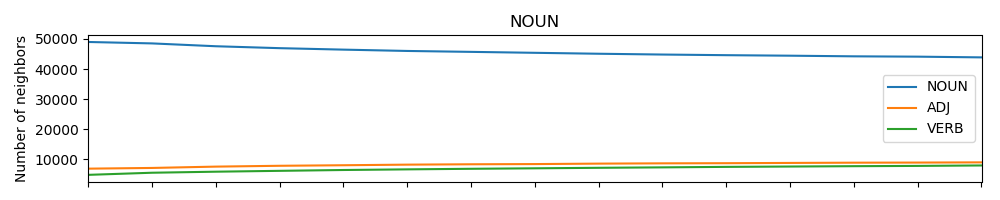
\includegraphics[width=\textwidth]{figs/NOUN_nn_100_fasttext_enwiki-20170501-clean_cbow-300d-min500_pos.png}
        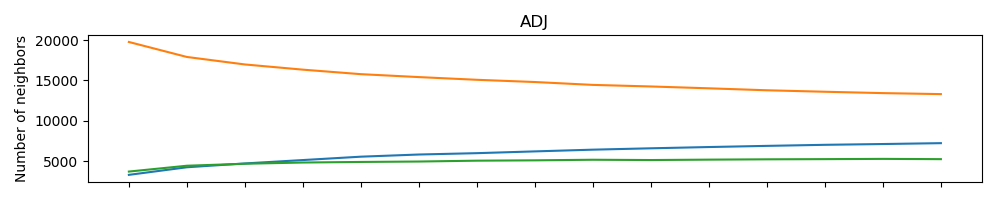
\includegraphics[width=\textwidth]{figs/ADJ_nn_100_fasttext_enwiki-20170501-clean_cbow-300d-min500_pos.png}
        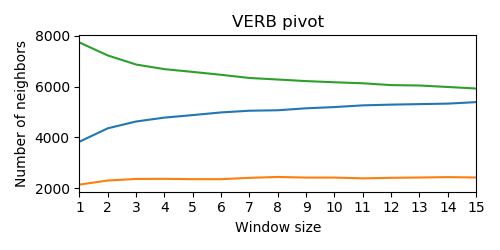
\includegraphics[width=\textwidth]{figs/VERB_nn_100_fasttext_enwiki-20170501-clean_cbow-300d-min500_pos.png}
	    \caption{Number of neighbor per POS for each pivot POS and for each window size.
	    The number of same-POS neighbors is consistently decreasing with window size.
	    \label{fig:nn_pos_hist}}
	\end{figure*}
    
    
    \section{Experiments}\label{sec:exp}
    
    \subsection{Data}\label{sec:data}
    We learn word embeddings from a corpus comprising all articles in English Wikipedia,
    using a dump from May 1, 2017\footnote{\url{https://dumps.wikimedia.org/enwiki}}.
    The data is preprocessed using a publicly available preprocessing
    script\footnote{\url{http://mattmahoney.net/dc/textdata.html}},
    extracting text, removing nonalphanumeric characters,
    converting digits to text, and lowercasing the text.
    
    \subsection{Hyper-parameters}\label{sec:hyperparams}
    We use fastText \cite{bojanowski2016enriching} to learn
    300-dimensional word embedding models,
    using the CBOW algorithm \cite{mikolov2013efficient}.
    The context window size varies from 1 up to 15.
    We set the minimal word occurrence count to 500, to avoid
    very rare words or uncommon spelling errors from skewing the results.
    All other hyper-parameters are set to their default values.
    
    To calculate the similarity between words, we use cosine similarity
    between their corresponding vectors.
    
    \subsection{Nearest Neighbor Analysis}\label{sec:nn_exp}
    	
    \paragraph{Collecting pivots.}
    
    We create a word list for each of the three most
    common parts of speech:
    nouns, adjectives and verbs\footnote{Our word lists will be released upon publication.}.
    For each POS, we list all lemmas of all synsets of that POS from
    WordNet \cite{miller1998wordnet}.
    To ``purify'' the lists and avoid noise from homonyms,
    we remove from each list any lemma that also belongs to a synset from
    another POS.
    As a further cleaning step, we use
    spaCy 2.0.11\footnote{\url{https://spacy.io}} (with the \texttt{en\_core\_web\_sm} model)
    to tag each word,
    and only keep words for which the spaCy POS agrees with the WordNet POS.
    Without context, spaCy will likely choose the most
    common POS based on its training corpus, which is different from WordNet,
    increasing the robustness of the combination.
    
    This process results in 6407 \textit{uniquely-noun}, 2784 \textit{uniquely-adjective}
    and 1460 \textit{uniquely-verb} words, which we refer to as our \textit{pivot lists}.
    
    \paragraph{Calculating nearest neighbor POS.}
    
    For each word in our pivot lists, we calculate the 100 nearest neighbors
    according to each learned word embedding model, filter these neighbors to
    keep only words in the spaCy vocabulary, and keep the top 10 valid neighbors.
    Again using spaCy, we tag the POS of each neighbor in the result.
    We subsequently calculate a histogram, for each POS $x$, of its
    \textit{neighbor-POS} $y$, that is, the POS assigned to the neighbors of
    words with POS $x$.
    
    \paragraph{Results.}
    
    Figure~\ref{fig:nn_pos_hist} shows the results of this experiment.
    For nouns, adjectives and verbs, we consistently see a decrease in
    the number of same-POS neighbors when we increase the window size,
    while other neighbors are increasing or unaffected.
    The Pearson correlations of the window size with the number of same-POS
    neighbors are $-0.96$, $-0.93$ and $-0.91$ for nouns, adjectives and verbs respectively,
    with $p<0.01$ (two-tailed t-test).
    
    \begin{table*}[ht]
    \centering
    \begin{tabular}{l|c|cc|cc|c}
    \hline
    && \multicolumn{2}{c|}{\bf \# Related} & \multicolumn{2}{c|}{\bf \# Unrelated} & \\
    \bf Benchmark & \bf Size & \bf All & \bf Same-POS & \bf All & \bf Same-POS & \bf p-value \\
    \hline
	WordSim353 & 353 & 122 & 107 & 53 & 40 & 0.038 \\
    WordSim353-S & 203 & 60 & 53 & 53 & 40 & 0.061 \\
    WordSim353-R & 252 & 104 & 89 & 39 & 31 & 0.26 \\
    SimLex999 & 999 & 234 & 199 & 334 & 295 & 0.897 \\
    RW & 2034 & 944 & 555 & 262 & 144 & 0.149 \\
    MEN & 3000 & 791 & 564 & 781 & 439 & $3\cdot10^{-10}$ \\
    MTurk287 & 287 & 49 & 39 & 119 & 68 & 0.004 \\
    MTurk771 & 771 & 204 & 153 & 200 & 146 & 0.365 \\
    SimVerb3500 & 3500 & 633 & 265 & 1217 & 566 & 0.974
    \end{tabular}
    \caption{Analysis of interchangeability (by same-POS) in
    word similarity and relatedness benchmarks.
    \label{tab:benchmark_results}}
    \end{table*}
    
    
    
    \subsection{Word Similarity Benchmark Experiments}\label{sec:benchmark_exp}
    
    \paragraph{Word similarity benchmarks.}
    
    To measure semantic word similarity, we use the following benchmarks:
    \begin{itemize}
        \item WordSim-353~\cite{finkelstein2001placing}
        \item WordSim-353-Sim~\cite{agirre2009study}
        \item WordSim-353-Rel~\cite{zesch2008using}
        \item SimLex999~\cite{hill2015simlex}
        \item Rare Word~\cite{luong2013better}
        \item MEN~\cite{bruni2012distributional}
        \item MTurk-287~\cite{radinsky2011word}
        \item MTurk-771~\cite{halawi2012large}
        \item SimVerb-3500~\cite{Gerz2016emnlp}
    \end{itemize}
    See Table~\ref{tab:benchmark_results} for the size of each benchmark.
    
    \begin{figure*}[ht]
        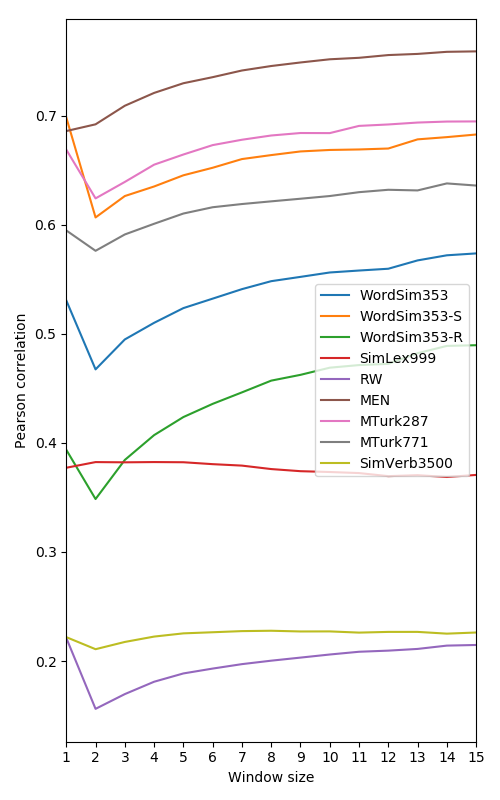
\includegraphics[width=\textwidth]{figs/distances_fasttext_enwiki-20170501-clean_cbow-300d-min500_eval.png}
	    \caption{Pearson correlation between benchmark score and word embedding cosing similarity,
	    for each benchmark and window size.
	    \label{fig:nn_pos_hist}}
	\end{figure*}

    \paragraph{Relatedness threshold.}
    
    While all of these benchmarks assign a score along a scale to each pair
    (calculated from human scoring), for our experiment we would like to use
    a binary annotation of whether a pair is related or not.
    For this purpose, we divide the whole range of scores,
    for each benchmark, to three parts:
    the lowest 30\% of the range between the lowest and highest scores
    is considered ``unrelated'', the top 30\% as ``related'',
    and the middle 40\% are ignored.
    
    Given the binary classification obtained from the human-annotated scores
    for each benchmark, we can find the enrichment of same-POS pairs among
    related pairs.
    Again, we use spaCy to annotate the POS for each word in each benchmark
    pair (tagging them in isolation to select the most probably POS),
    and look at the set of same-POS pairs in the benchmark.
    For each of the benchmark, we calculated a p-value using the hypergeometric
    test, comparing the enrichment of same-POS pairs within related pairs,
    with a background of all related and unrelated pairs (ignoring ones in
    the middle 40\% range of scores).
    
    Table~\ref{tab:benchmark_results} shows the results of this division.
    For WordSim353, MEN and MTurk287, the set of related pairs
    contains significantly more same-POS pairs than the background set.
    In SimLex999 and in SimVerb3500, all pairs are same-POS by design:
    in SimVerb all words are verbs, and in SimLex every pair is of the same POS.
    The fact that not all pairs in these benchmarks are judged as same-POS
    in our experiment is due to ambiguity: for some words, spaCy selected a POS
    which is not the one intended in constructing the benchmark.
    
    \paragraph{Relation to window size.}
    
    To investigate the effect of window size on a model's performance on the benchmark
    datasets, we evaluate each model on each benchmark, again using cosine similarity
    as the model's prediction for each pair.
    Interestingly, we see a positive correlation of window size with model's performance
    for WordSim353, WordSim353-R, MEN, MTurk287, and MTurk771 (with $p<0.01$; two-tailed t-test).
    For SimLex999, we see a negative correlation instead ($p<0.01$).
    
    

\section{Discussion}\label{sec:discussion}

The same analysis could be applied to the vector dimension.

    \bibliographystyle{acl_natbib}
    \bibliography{references}
\end{document}
